\documentclass[a4paper, 12pt]{article}

\usepackage[T2A]{fontenc}
\usepackage[utf8]{inputenc}
\usepackage[russian]{babel}
\usepackage{geometry}
\usepackage{setspace}
\usepackage{hyperref}
\usepackage{listings}
\usepackage{graphicx}
\usepackage{indentfirst}
\usepackage{titlesec}
\usepackage{pgfplots}
\usepackage{pgfplotstable}

\pgfplotsset{width=12cm, compat=1.18}
\newgeometry{left=1.5 cm, right=1.5cm, top=1.5cm, bottom=1.5cm}

\begin{document}


% ---------------------------------- Титульник ----------------------------------
\hypersetup{pageanchor=false}
\begin{titlepage}
 \begin{center}
  \vspace*{1cm}

  \Huge
  \textbf{Лабораторная работа №2}

  \vspace{0.5cm}
  \LARGE
  ``Выделение ресурса параллелизма. Технология OpenMP''

  \vspace{1.5cm}
  Выполнил студент группы Б20-505\\
  \textbf{Сорочан Илья}

  \vfill

  \Large
  Московский Инженерно-Физический Интститут\\
  Москва 2023

 \end{center}
\end{titlepage}


% ---------------------------------- Рабочая среда ----------------------------------

\section{Рабочая среда}

Технические характеристики (вывод \textit{inxi}):
\begin{verbatim}
CPU: 6-core AMD Ryzen 5 4500U with Radeon Graphics (-MCP-)
speed/min/max: 1396/1400/2375 MHz Kernel: 5.15.85-1-MANJARO x86_64 Up: 46m
Mem: 2689.5/7303.9 MiB (36.8%) Storage: 238.47 GiB (12.6% used) Procs: 238
Shell: Zsh inxi: 3.3.24
\end{verbatim}

Используемый компилятор:
\begin{verbatim}
gcc (GCC) 12.2.0
\end{verbatim}

Согласно \href{https://www.openmp.org/resources/openmp-compilers-tools/}{официальной документации} даная версия компилятора поддерживает \textit{OpenMP 5.0}

% ---------------------------------- Анализ алгоритма ----------------------------------

\section{Анализ алгоритма}

Данный алгоритм ищет индекс заданного элемента в массиве со случайно сгенерирированными значениями.\\
Временная сложность:
\begin{itemize}
 \item В лучшем случае -- $O(1)$;
 \item В хужшем -- $O(count)$, где $count$ количество элементов в массиве.
\end{itemize}

Хочу так же заметить, что хоть и маловероятно, но программа может не найти элемент с заданным значеним. Данный случай никак не обрабатывается выданном коде. В параллелизованом производится замер времени, соответсвенно результат вычислений не представляет интереса.

Так же важно то, что в предоставленной программе память, выделенная под массив не была освобождена. Это исправлено в новой версии программы.

\vspace{0.5cm}

Блок схема поиска элемента:\\
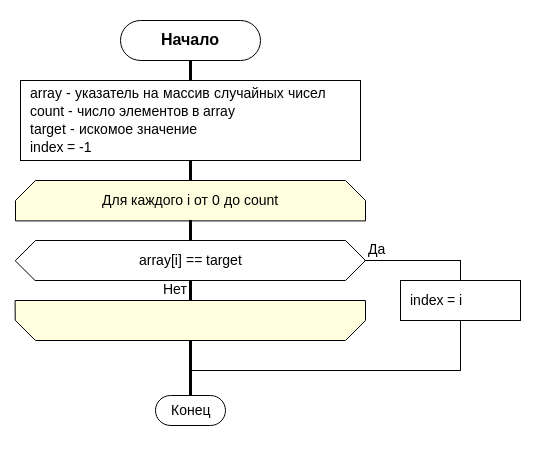
\includegraphics[scale=0.6]{res/original.png}


% ---------------------------------- Параллелизация ----------------------------------

\section{Параллелизация}

Очевидно, что наиболее тяжелым структурным элементом является цикл алгоритма.

Для начала зададим несколько опций параллелизации с помощью \textit{omp parallel}:
\begin{itemize}
 \item \textit{num\_threads} - число используемых потоков;
 \item \textit{shared(array, count, index, target)} - общая для всех потоков память (переменные). Сюда включены массив, его размер, индекс искомого элемента (для сохранения результата) и искомое значение соответсвенно;
 \item \textit{default(none)} - локальность всех переменных, не указанных в \textit{shared}.
\end{itemize}

Перед самим циклом поставим \textit{omp for} для распределения его итераций между потоками. При этом не забудем заменить \textit{break} на \textit{omp cancel for}. Эта директива прервет исполнение всех потоков, если мы найдем искомый элемент.

Важно заметить, что для работы \textit{omp cancel for} при запуске необходимо устанавливать значение переменной окружения \textit{OMP\_CANCELLATION=true}.

Еще была добавлена директива \textit{omp critical} для того, что бы присваивание в общую переменную \textit{index} производилось последовательно в разных потоках.

В итоге каждый поток будет по сути придерживатся той же блок схемы, за исключением двух деталей:
\begin{itemize}
 \item $i$ меняется от $\frac{count}{threads} \cdot tid$ до $\frac{count}{threads} \cdot (tid + 1)$, где $count$ число элементов в массиве, $threads$ -- число потоков;
 \item При обнаружении искомого элемента все потоки прерываются.
\end{itemize}


% ---------------------------------- Графики ----------------------------------

\section{Экспериментальные данные}

Во всех измерениях бралось 10 запусков на поток.

\vspace{0.3cm}

\begin{tikzpicture}
 \begin{axis}[
    xlabel={Число потоков},
    ylabel={Время (мс)},
    legend pos=north east,
  ]
  \addplot table [x=Threads, y=Worst (ms), col sep=comma] {data/data.csv};
  \addplot table [x=Threads, y=Best (ms), col sep=comma] {data/data.csv};
  \addplot table [x=Threads, y=Average (ms), col sep=comma] {data/data.csv};
  \legend{Худшее время, Лучшее время, Среднее время}
 \end{axis}
\end{tikzpicture}

\vspace{0.5cm}

Из графика видно, что в среднем многопоточная программа работает медленнее. Я могу выделить две основные причины.

Во-первых представленная задача проста в вычислительном плане. Вполне возможно, что инициализация работы с потоками и их прерывание занимают слишком много времени для такой тривиальной задачи.

Во-вторых оптимизации компилятора. Я провел повторные тесты с добавлением флага \textit{-O3}:

\vspace{0.3cm}

\begin{tikzpicture}
 \begin{axis}[
    xlabel={Число потоков},
    ylabel={Среднее время (мс)},
    legend pos=north east,
  ]
  \addplot table [x=Threads, y=Worst (ms), col sep=comma] {data/optimized.csv};
  \addplot table [x=Threads, y=Best (ms), col sep=comma] {data/optimized.csv};
  \addplot table [x=Threads, y=Average (ms), col sep=comma] {data/optimized.csv};
  \legend{Худшее время, Лучшее время, Среднее время}
 \end{axis}
\end{tikzpicture}

\vspace{0.3cm}

Прекрасно видно, что однопоточная программа лидирует с большим отрывом и причиной этому -- оптимизации компилятора.

Для сравнения вот среднее время с \textit{-O3} и без него:

\vspace{0.3cm}

\begin{tikzpicture}
 \begin{axis}[
    xlabel={Число потоков},
    ylabel={Среднее время (мс)},
    legend pos=north east,
  ]
  \addplot table [x=Threads, y=Average (ms), col sep=comma] {data/data.csv};
  \addplot table [x=Threads, y=Average (ms), col sep=comma] {data/optimized.csv};
  \legend{Без \textit{-O3}, C \textit{-O3}}
 \end{axis}
\end{tikzpicture}

\vspace{0.3cm}

Рассмотрим так же прирост, даваймый каждым числом процессоров относительно первого (берем среднее время):

\begin{tikzpicture}
 \begin{axis}[
    xlabel={Число потоков},
    ylabel={Прирост (\%)},
    ybar interval=0.7,
  ]
  \addplot table [x index=0, y index=1, col sep=comma] {data/compare.csv};
 \end{axis}
\end{tikzpicture}

% ---------------------------------- Заключение ----------------------------------

\section{Заключение}
В данной работе было исследовано ускорение, получаемое при использовании многопоточности в задании о нахождении максимума. Была усовершенствована предоставленная программа и написан специальный скрипт, собирающие данные о нескольких запусках этой программы в один файл, попутно её перекомпилируя.

В ходе работы было выяснено, что в данной задаче применение многопоточности лишь замедлит программу. С уверенностью можно сказать, что частью причины таких результатов являются оптимизации, производимые компилятором.

С другой стороны стоит отметить, что вычислительная сложность программы низка, а соответсвенно инициализация потоков не выгодна.

\appendix

\titleformat{\section}[display]
  {\normalfont\Large\bfseries}
  {\centering Приложение\ \thesection\\}
  {0pt}{\Large\centering}
\renewcommand{\thesection}{\Asbuk{section}}

\section{Использованные программные коды}

Оригинальный предоставленный код:
\lstinputlisting[language=C, basicstyle=\tiny]{src/original.c}
\vspace{0.5cm}

Код без многопоточности:
\lstinputlisting[language=C, basicstyle=\small]{src/main.c}
\vspace{0.5cm}

Доработанный код:
\lstinputlisting[language=C, basicstyle=\tiny]{src/threaded.c}
\vspace{0.5cm}

Для сборки данных использовался следующий скрипт:
\lstinputlisting[language=Python, basicstyle=\tiny]{src/main.py}
\vspace{0.5cm}

Для вычисления относительного прироста производительности использовался следующий скрипт:
\lstinputlisting[language=Python, basicstyle=\footnotesize]{src/compare.py}
\vspace{0.5cm}

\section{Таблицы с теоритическими и практическими результатами}

Таблица без оптимизаций:

\vspace{0.3cm}

\pgfplotstabletypeset[
 col sep=comma,
 columns={Threads,Worst (ms),Best (ms),Average (ms)},
]{data/data.csv}

\vspace{0.5cm}

Таблица с оптимизациями:

\vspace{0.3cm}

\pgfplotstabletypeset[
 col sep=comma,
 columns={Threads,Worst (ms),Best (ms),Average (ms)},
]{data/optimized.csv}

\vspace{0.5cm}

Таблица сравнений:

\vspace{0.3cm}

\pgfplotstabletypeset[
 col sep=comma,
 columns={Threads,Efficiency},
]{data/compare.csv}


\end{document}
